\documentclass[journal]{IEEEtran}
\usepackage{eurosym}
\ifCLASSINFOpdf
  \usepackage[pdftex]{graphicx}
  \DeclareGraphicsExtensions{.pdf,.jpeg,.png}
\else
   \usepackage[dvips]{graphicx}
 \fi
\usepackage{subfig}
 \let\MYorigsubfloat\subfloat
 \renewcommand{\subfloat}[2][\relax]{\MYorigsubfloat[]{#2}}
\usepackage{url}
\hyphenation{}
\usepackage{float}

\begin{document}
\title{Design of 1Mbit RRAM memory to replace eFlash}
\author{Diels Wouter, Standaert Alexander}% <-this % stops a space
\markboth{KULeuven Master Thesis, May 2014}%
{Evaluation paper}

\maketitle


\begin{abstract}
%%%%%%%%%%%%%%%%%%%%%%%%%%%%%%%%%%%%%% Write abstract
A 1Mbit RRAM memory in 45nm technology is presented. The focus lies on read reliability. To overcome variability a tunable reference signal is generated by connecting multiple reference cells in parallel. A bitline load has been designed to optain maximum bitline voltage difference. Sense amplifier performance has been improved by allowing overlap between passgate-enable and latch-enable signals, this overlap gives rise to a nonlinear phenomenon, the RC-latch-effect. Write operation has not been included in the design and the results are based on circuit simulations.
\end{abstract}
\hfill May 20, 2014

\section{Introduction}

\IEEEPARstart{N}{on}-volatile memories such as flash are widely used for mass storage devices, but are also steadily finding their way into the embedded domain. However, as discussed in \cite{Pra10}, it is getting difficult to fabricate reliable flash memories in diep-submicron. It is argued that the scaling of flash-memories will not last for more than a few technology nodes. RRAM memories, in which information is stored in the resistive state of a memristor, would be able to scale futher, due to the fact that it is a nanopartical based memory\cite{rramscaling}. Furthermore, the memristor fabrication can easily be integrated in a standard CMOS fabrication process. In this work, a RRAM memory has been designed, armed against intra-die variations. A read access time of 2.3ns and an energy consumption of 0.51pJ makes it faster and less energy gready than conventional flash memories.
This paper is structured as follows: Section \ref{Genach} discusses the general architecture, this is the way the 1T1R cells are put together. In section \ref{ref}, the tuning of the reference voltage will be explained. Section \ref{load} will present the results of the load analysis, in which an optimal load impedance is chosen for sufficiently large voltage differences for the sense amplifier and sufficiently low voltage drops over the memristor. In section \ref{sens}, some techniques for decreasing the offset voltage of the sense amplifier will be explained. Finally (Section \ref{final}) the results of the completed circuit will be presented.


\section{General architecture}\label{Genach}
The general architecture can be seen in figure \ref{fig:architecture}. The memory consist of 512 global blocks (GB). Each GB consists of two local blocks (LB), which in turn consists of 32 bitlines (BL) and sourcelines (SL) and 32 wordlines (WL). A branch is defined as a collection of memory cells connected to one BL and one SL.

\subsection{Branch}
In a branch 32 1T1R cells are connected to a BL and a SL. The transistor terminal of the cell is connected to the SL and the memristor terminal of the cell is connected to the BL. The memristors can be either HRS or LRS. Besides these 32 data cells, there is also one reference cell in the branch, its gate is connected to the reference WL. Connected to the BL is a load. The load consists out of a single pMOS transistor that is connected to the supply voltage, which is switched on and off by means of logic. Also connected to the BL is a nMos transistor that serves as a switch to the ground voltage. An nMOS switch is also placed between the SL and the ground voltage. This switch is needed if a write circuit is implemented so that the current can also flow in reverse direction though the memristor.

\begin{figure}[b!]
  \centering
  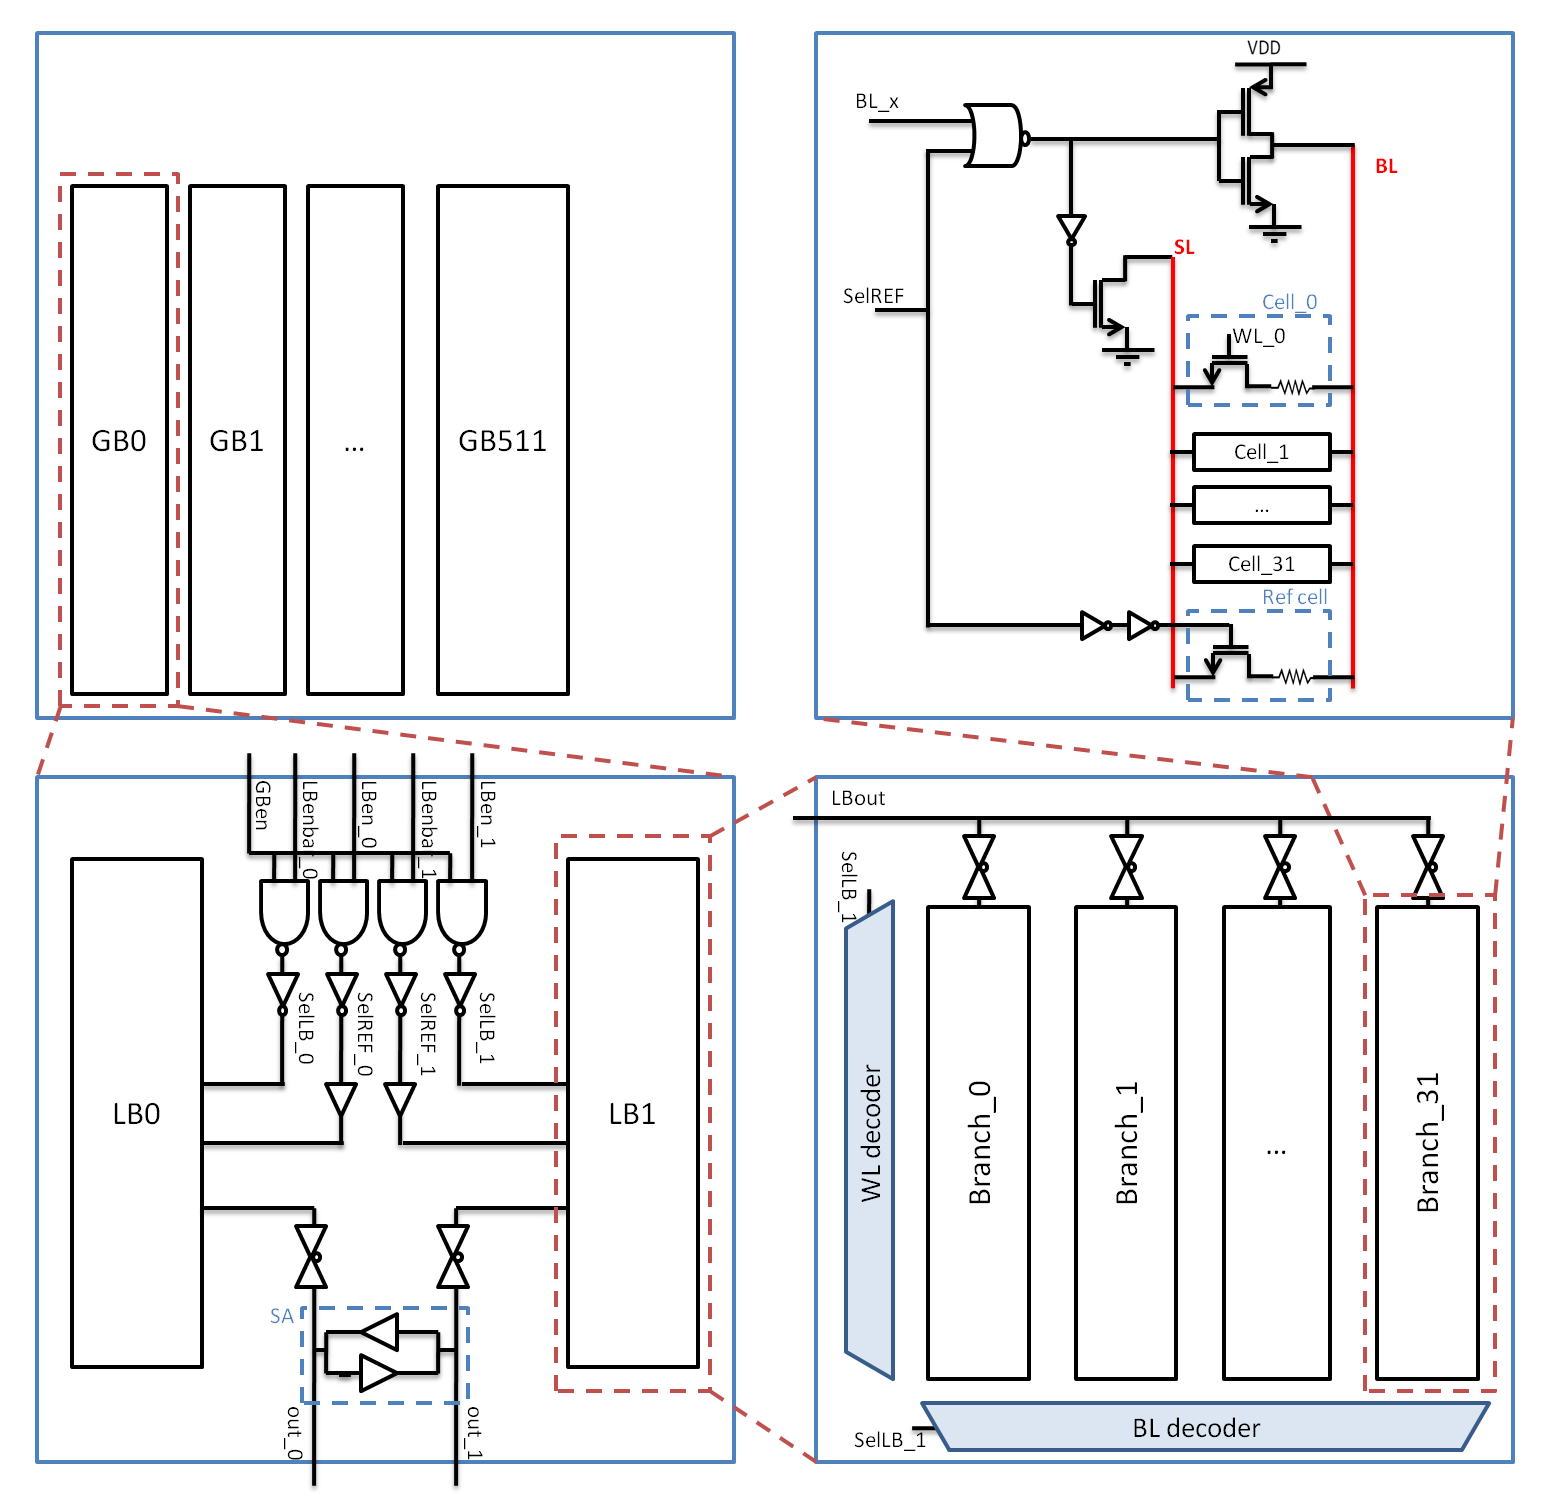
\includegraphics[width=0.5\textwidth]{../fig/paper-architecture.png}
  \caption{Overview architecture}
  \label{fig:architecture}
\end{figure}

\subsection{Local block}
A local block (LB) consists of 32 branches, BL \& WL decoder and passgates on the BL of each branch (BL mux). The passgates are connected to the output node LBout. To read out a data cell, the appropriate WL is brought to the supply voltage. The BL-load and SL-transistor of the apporopriate BL and SL are switched on. A current will flow from the supply voltage through the load, the cell and SL-switch to the ground voltage and a voltage will appear on the BL node. The pass-gate of the BL is then turned on and the BL voltage is passed to the output of the LB. Reference signals are generated by activating the reference WL and turning the BL loads and SL switches on. The BLs are then shorted by turning on all the appropriate passgates. This averages the BL voltages to a signal which has a value between the BL voltage of a cell in HRS and LRS. To save energy, not all 32 reference cells in a LB are used to generate the reference signal.

\subsection{Global block} 
A global block (GB) consists out of two LBs and a sense amplifier. If one LB produces a data signal at its output, the other will produce a reference signal and vice versa. While reading a cell in the memory cicuit, only one GB is active. This is garantied by the GBen signal.


\section{Tuning the reference signal distribution}\label{ref}
Due to intra-die variations, the properties of different components in the circuit vary. In this work, variations of the transistor parameters $V_{T}$ and $\beta$ are considered and modelled with normal distributions. The variations of the resistive value of the memristor are also considered, normal distributions are used to model both HRS and LRS. Due to these component variations, signals such as the data and reference signal also have a distribution. The distribution of the reference signal however, can be tuned in contrast to the data signal. Recall that the reference signal is generated by shorting active BLs using passgates. Shorting a BL with an addressed HRS reference cell with a BL with a LRS reference cell would suffice for producing a voltage lying between a HRS data voltage and a LS data voltage. By using this shorting technique however the mean of the reference signal PDF would not lie exactly between the means of the HRS data PDF and LRS data PDF. By implementing more than 2 reference cells for the reference signal, and having more HRS (LRS) cells than LRS (HRS) cells, the mean of the reference signal PDF can be shifted. Furthermore, the distribution will have a smaller spread by implementing a bigger amount of reference cells. One should not implement too many reference cells however, since energy consumption (for each active reference cell, current flows through its corresponding bitline) increases drastically. In this design 16 reference cells in a LB are addressed for generating the reference signal, the remaining 16 serve as dummies. Of the 16 active reference cells, 6 are HRS and 10 are LRS.

\section{Load analysis}\label{load}
Due to the aforementioned variations in the circuit, the data and reference signals should be designed in such a way that they are sufficiently far apart. The minimal distance of these two signals directly influence the minimal offset the SA should have. Moreover, the distributions of these signals cannot overlap or a correct reading of the cell will not occure. The load impedance influences the value of the data and reference voltages, it also determines the settling time of the charging of the BL and the voltage drop over the memristor. Destructive reads might occur because of a to high voltage drop over the memristor. As it turns out, fast settling is not compatible with low memristor voltage drop and large voltage difference. Because the latter are imperative for a reliable memory and the former is not, settling time had no bearing on the final choice of load impedance. Several different types of load were considered \cite{bulkload} but the best performance with variability was achieved with a single transistor load. Figure \ref{fig:switchloadresults} shows nominal HRS/LRS voltage differences and memristor voltage drop for several pMOS transistor loads with different sizes. 

\begin{figure}[ht!]
  \centering
  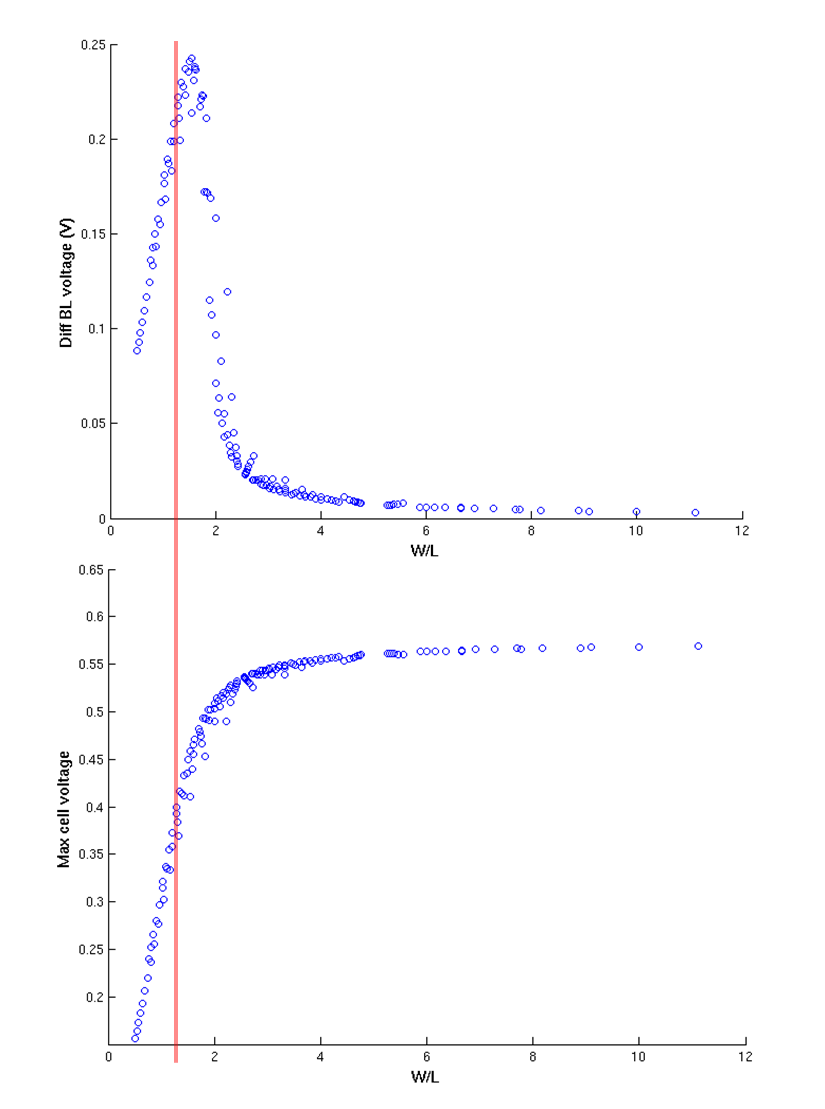
\includegraphics[width=0.4\textwidth]{../fig/hfdst-last-length.png}
  \caption{Nominal HRS/LRS BL voltage difference and voltage drop over memristor for pMOS transistor loads}
  \label{fig:switchloadresults}
\end{figure}

In the end a transistor with a width of 300nm and a length of 198nm was chosen. In figure \ref{fig:distributions} the distributions of the data and reference voltages are displayed for this load.

\begin{figure}[ht!]
  \centering
  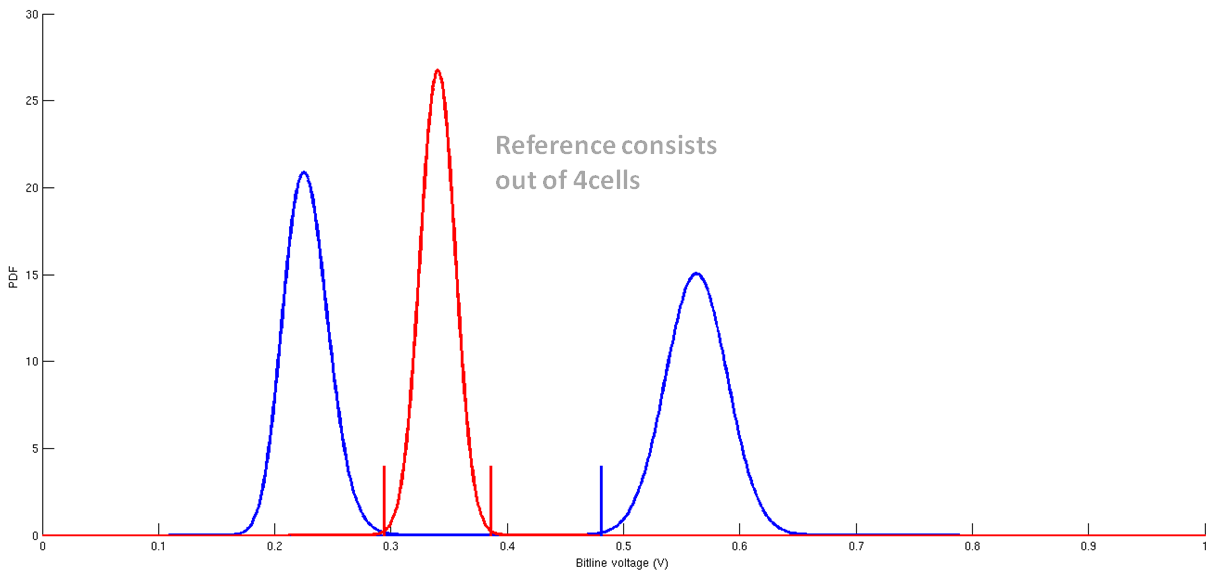
\includegraphics[width=0.4\textwidth]{../fig/hfdst-last-var2.png}
  \caption{Distributions of the reference signal and HRS \& LRS data signals }
  \label{fig:distributions}
\end{figure}

\section{Sense amplifier overlap techniques}\label{sens}
This design uses the drain-input latch-type SA (see figure \ref{fig:ourSA}). Its input/output nodes are connected to the output nodes of the local block through complementary passgates. There are two ways to implement the latch timing cycle: one could separate the pass operation from the latch operation or could allow overlap between these two operations.

\begin{figure}[ht!]
  \centering
  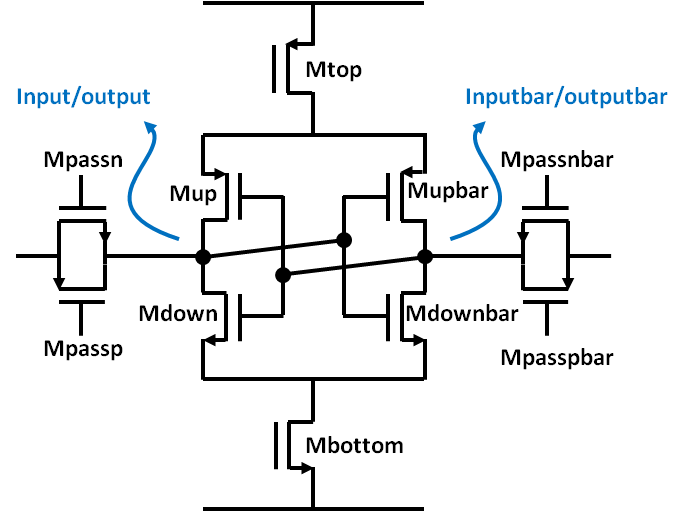
\includegraphics[width=0.25\textwidth]{../fig/hfdstk-sensamp-ourSA2.png}
  \caption{Drain-input latch-type sense amplifier\cite{Cos09} used in this design}
  \label{fig:ourSA}
\end{figure}


\subsection{No overlap: disconnect inputs before activating current source}
The SA can be activated after the pass-gates are disconnected. Using this control scheme, the SA would be separated from the local block when enabled. Offset voltage spread is mainly determined by the $\Delta_{V_{T}}$ and $\Delta_{\beta}$ variations of the differential pairs of the SA. These contributions can be decreased by increasing the sizes of the differential pair transistors. Sizing up the top and bottom transistor has more influence on the latching speed rather than the offset voltage. There is also a slightly surprising contribution on the offset voltage by the passgates. This can be explained by the charge injection of the passgates: when the passgates are turned on, the output voltage of the local block is passed on to the input/output node of the SA almost perfectly - whether there are variations on the transistors or not. When the passgates are turned off, a charge injection occurs on the SA input/output node - distorting the original voltage. The SA operates differentially though, so as long as this charge injection is matched at the two input/output nodes there would be no problem. $\beta$ mismatch of the passgate transistors however results in charge injection mismatch (see figure \ref{fig:chargeinjection}). Hence the contribution of the passgates to the offset voltage spread. This mismatch can be reduced by sizing up the passgates transistors. More charge is injected when the passgates are turned off, but the distortion difference at the two sides is reduced. This reduces the offset contribution of the passtransistors.

\begin{figure}[ht!]
  \centering
  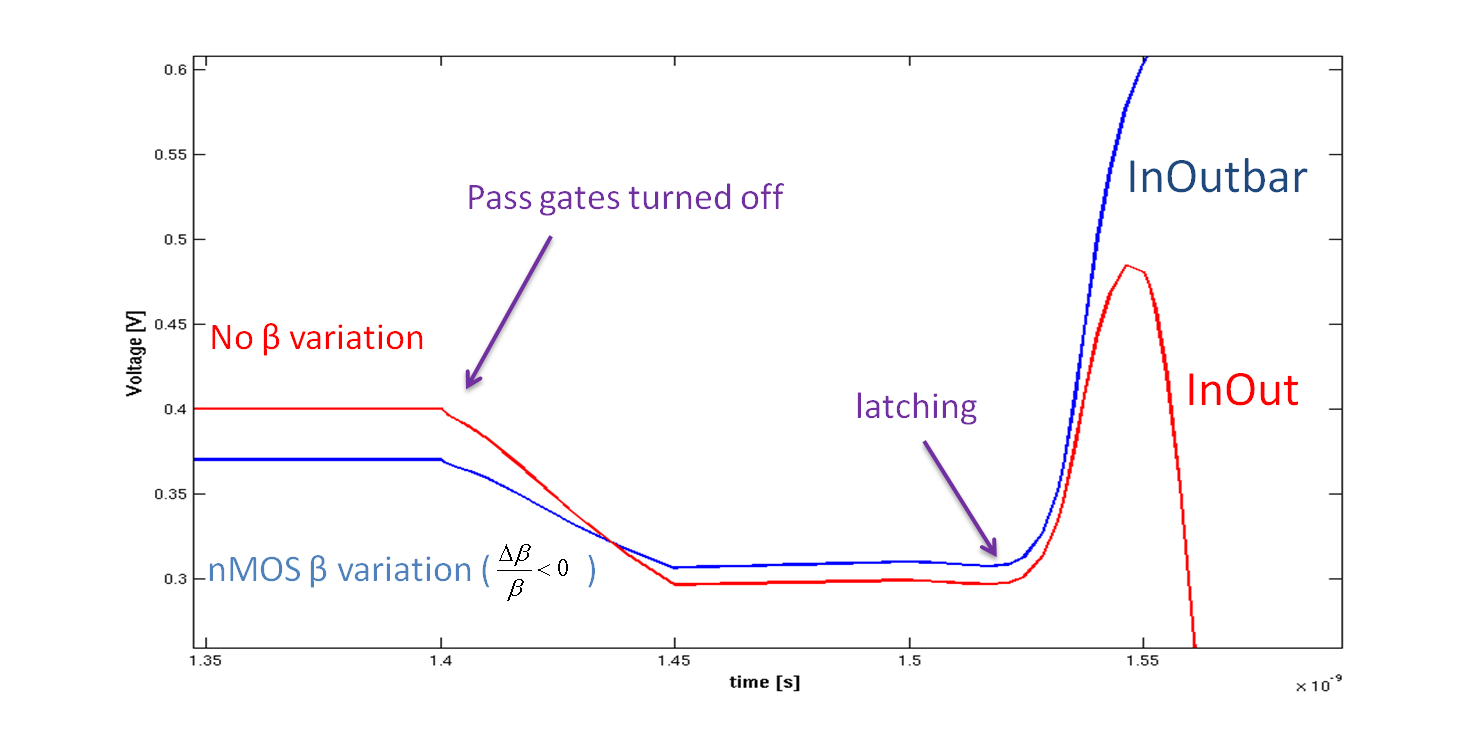
\includegraphics[width=0.5\textwidth]{../fig/hfdstk-sensamp-chargeinjectionmismatch.png}
  \caption{Charge injection mismatch due to $\beta$ variations of passgate transistors}
  \label{fig:chargeinjection}
\end{figure}

\subsection{Overlap: inputs are connected when current source is activated}
If the passgates are still turned on when the SA starts latching, the voltage difference of the input/output nodes has not experienced charge injection mismatch. When the voltage difference has been sufficiently amplified, the passgates are turned off. Charge injection (mismatch) will occur, but it will not change the outcome of the latching anymore. During the overlap of the pass and latching operation, the passgates can be modeled by resistors. Neglecting the capacitance of the output node (LBout) of the local block, the situation can be depicted as in figure \ref{fig:RC-latch}. CL is the bitline capacitance.

\begin{figure}[ht!]
  \centering
  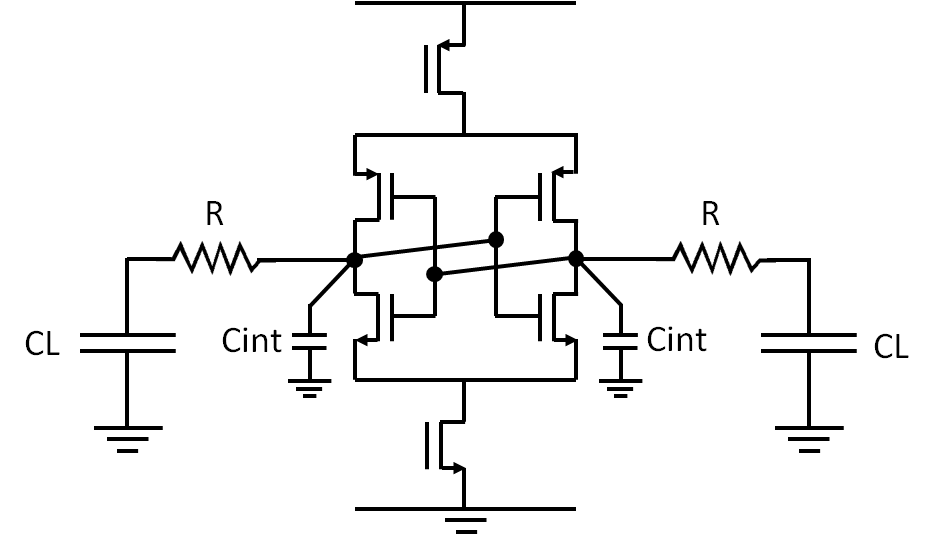
\includegraphics[width=0.25\textwidth]{../fig/hfdstk-sensamp-RC-latch.png}
  \caption{Simplified circuit when overlap between pass enable and latch enable is applied}
  \label{fig:RC-latch}
\end{figure}

One could suspect that a large BL capacitance would significantly increase the latching time. While this is true for small values of R, as can be seen in figure \ref{fig:RC-latch-sim}, for greater values the latching goes through two phases: during the first phase, it appears as if the big capacitance is decoupled from the SA. After this fast phase, settling is much slower. 

\begin{figure}[ht!]
  \centering
  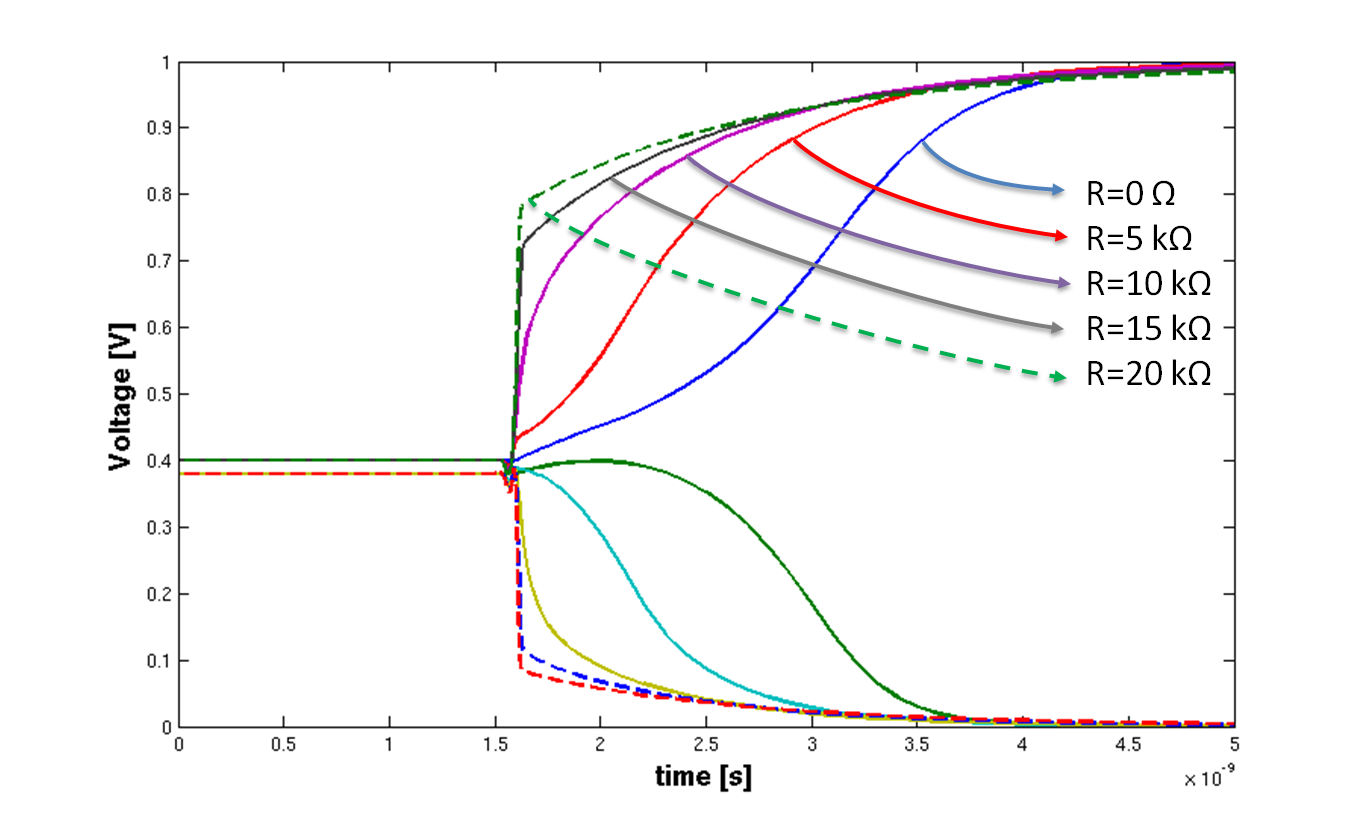
\includegraphics[width=0.5\textwidth]{../fig/hfdstk-sensamp-RC-latch-sim.png}
  \caption{Transient simulation for the schematic of figure \ref{fig:RC-latch} for different values of R, CL = 46fF, SA is minimal, no variations are included in simulation}
  \label{fig:RC-latch-sim}
\end{figure}

This RC-latch effect arises when the RC-product of the pass-gate resistance and the BL capacitance is large. When it occurs, the capacitance behaves as a short-circuit and current flows through the resistor and a corresponding voltage drop over the resistor builds up. Afterwards the load capacitance charges itself at a much lower time constant.\\\\
The overlap between the enabling of the passgates and the SA thus needn't be this great: a load-less SA latching delay suffices. For this situation $V_{T}$ and $\beta$ mismatch of the passgate transistors results in mismatch of the resistors. The interaction between these resistors and the SA is strongly non-linear. Depending on the precharged values of the load capacitances, this R mismatch can result in incorrect latching. There is thus still a contribution of the passgates to the offset voltage spread. The interaction between R and the SA reduces the contributions of the differential pair mismatch however. For a minimal SA, the offset voltage spread is smaller with overlap than without. By sizing all the transistors, this spread can be reduced to the desired level. Speed can be improved by using the RC-latch effect which implies using small pass-gate transistors, or by sizing the rest of the SA. This allows the SA to deliver a large current to charge the BL capacitance.

\section{Read Throughput Results}\label{final}
A read access time simulation test was performed on the completed circuit (Figure \ref{fig:speedvdd}). In this test the supply voltage was decreased and the maximum read throughput was measured. The test was performed at a (SPICE enviroment) temperature of $30^{\circ}\mathrm{C}$. At each point in the shmoo plot, 100 MonteCarlo simulations were performed. At 1V Vdd, the circuit achieves a read access time of 2.3ns. during the read cycle, its energy consumption is 0.51pJ. Most of the energy (65\%) is consumed by the bitlines. 25\% of the energy consumption is due to the logic, while the buffers and SA together take the remaining 10\%. As the supply voltage goes down, the read throughput also goes down. This is caused by a combination of phenomena. First of all the logic operates slower. This causes a timing issue in which the bitline load transistor is activated before the cell. This timing issue results in a rapid increase in bitline voltage which causes a longer settling time of the bitline when the cell is eventually selected. A second reason for the decrease in read throughput at a lower supply voltage, is the slower latching of the SA.

\begin{figure}[h!t]
  \centering
  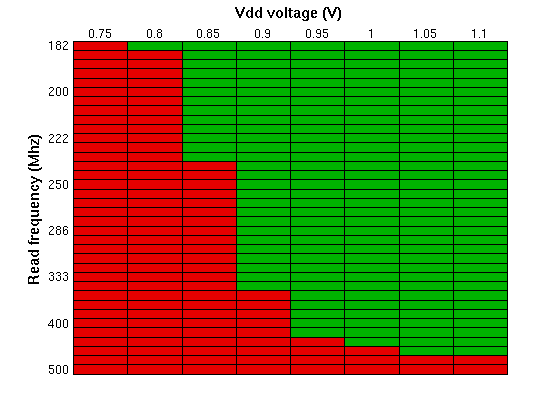
\includegraphics[width=0.5\textwidth]{../fig/hfdst-final-vddspeed.png}
  \caption{Results read access time test. Green succesful simulation. Red unsuccesful simulation}
  \label{fig:speedvdd}
\end{figure}

On figure \ref{fig:speedvdd} it can clearly be seen that the circuit can only operate down to a supply voltage of $0.8V$. An explanation for this is given in figure \ref{fig:vblvdd}. As vdd is decreased, the bitline voltage distributions of the reference signal and HRS \& LRS data signals also decrease. Eventually the bitline voltage distributions overlap and there is a high probability of circuit failure.

\begin{figure}[h!t]
  \centering
  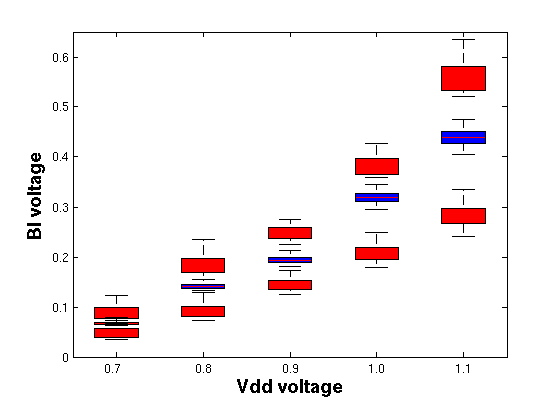
\includegraphics[width=0.5\textwidth]{../fig/hfdst-final-vddbl.png}
  \caption{BL voltage distribution for reference signal and HRS \& LRS signals in function of vdd}
  \label{fig:vblvdd}
\end{figure}




\section{Conclusion}
A 1Mb RRAM memory has been designed and presented. This memory design employs several techniques to improve performance and reliability. A good reference voltage distribution was achieved by averaging the signal from 10LRS and 6HRS cells. A load impedance was carefully chosen to maximize HRS \& LRS voltage differences while keeping the memristor voltage drop sufficiently low to avoid resistive switching and thus distructive reading. Overlap between passgates and sense amplifier operation reduces offset voltage spread as it avoids differential charge injection. Although keeping the passgates enabled while activating the SA does mean currrent flows from SA to BL, the impact of this on SA speed and energy is small, as Rpassgate*CBL is much larger than the overlap time..


\bibliography{references}{}
\bibliographystyle{IEEEtran}



\end{document}


\begin{thebibliography}{0}



\end{thebibliography}
%
